%% автогенерация: scripts/figures_tex.py — руками не править
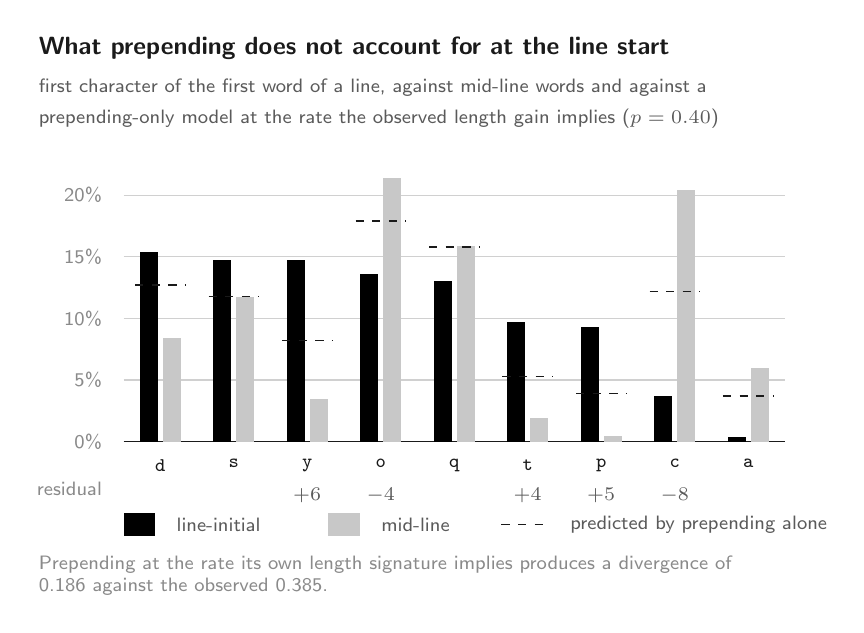
\begin{tikzpicture}[x=1mm,y=1mm,font=\sffamily\scriptsize]
\definecolor{ink}{HTML}{1A1A1A}\definecolor{inkii}{HTML}{5A5A5A}
\definecolor{inkiii}{HTML}{8A8A8A}\definecolor{rule}{HTML}{D0D0D0}
\definecolor{fill}{HTML}{2B2B2B}\definecolor{fillii}{HTML}{9A9A9A}
\definecolor{filliii}{HTML}{C8C8C8}
\node[anchor=west,font=\sffamily\small\bfseries,text=ink] at (0,64) {What prepending does not account for at the line start};
\node[anchor=west,text=inkii] at (0,59) {first character of the first word of a line, against mid-line words and against a};
\node[anchor=west,text=inkii] at (0,55) {prepending-only model at the rate the observed length gain implies ($p=0.40$)};
\draw[ink] (12,14.00) -- (96,14.00);
\node[anchor=east,text=inkiii] at (10.5,14.00) {0\%};
\draw[rule] (12,21.83) -- (96,21.83);
\node[anchor=east,text=inkiii] at (10.5,21.83) {5\%};
\draw[rule] (12,29.65) -- (96,29.65);
\node[anchor=east,text=inkiii] at (10.5,29.65) {10\%};
\draw[rule] (12,37.48) -- (96,37.48);
\node[anchor=east,text=inkiii] at (10.5,37.48) {15\%};
\draw[rule] (12,45.30) -- (96,45.30);
\node[anchor=east,text=inkiii] at (10.5,45.30) {20\%};
\fill[fill] (14.07,14) rectangle (16.37,38.10);
\fill[filliii] (16.97,14) rectangle (19.27,27.15);
\draw[ink,line width=.5pt,dashed] (13.47,33.88) -- (19.87,33.88);
\node[below,font=\ttfamily\scriptsize,text=ink] at (16.67,13) {d};
\fill[fill] (23.40,14) rectangle (25.70,37.01);
\fill[filliii] (26.30,14) rectangle (28.60,32.31);
\draw[ink,line width=.5pt,dashed] (22.80,32.47) -- (29.20,32.47);
\node[below,font=\ttfamily\scriptsize,text=ink] at (26.00,13) {s};
\fill[fill] (32.73,14) rectangle (35.03,37.01);
\fill[filliii] (35.63,14) rectangle (37.93,19.48);
\draw[ink,line width=.5pt,dashed] (32.13,26.83) -- (38.53,26.83);
\node[below,font=\ttfamily\scriptsize,text=ink] at (35.33,13) {y};
\node[below,text=inkii] at (35.33,9.4) {$+6$};
\fill[fill] (42.07,14) rectangle (44.37,35.29);
\fill[filliii] (44.97,14) rectangle (47.27,47.50);
\draw[ink,line width=.5pt,dashed] (41.47,42.02) -- (47.87,42.02);
\node[below,font=\ttfamily\scriptsize,text=ink] at (44.67,13) {o};
\node[below,text=inkii] at (44.67,9.4) {$-4$};
\fill[fill] (51.40,14) rectangle (53.70,34.35);
\fill[filliii] (54.30,14) rectangle (56.60,38.89);
\draw[ink,line width=.5pt,dashed] (50.80,38.73) -- (57.20,38.73);
\node[below,font=\ttfamily\scriptsize,text=ink] at (54.00,13) {q};
\fill[fill] (60.73,14) rectangle (63.03,29.18);
\fill[filliii] (63.63,14) rectangle (65.93,16.97);
\draw[ink,line width=.5pt,dashed] (60.13,22.30) -- (66.53,22.30);
\node[below,font=\ttfamily\scriptsize,text=ink] at (63.33,13) {t};
\node[below,text=inkii] at (63.33,9.4) {$+4$};
\fill[fill] (70.07,14) rectangle (72.37,28.56);
\fill[filliii] (72.97,14) rectangle (75.27,14.78);
\draw[ink,line width=.5pt,dashed] (69.47,20.10) -- (75.87,20.10);
\node[below,font=\ttfamily\scriptsize,text=ink] at (72.67,13) {p};
\node[below,text=inkii] at (72.67,9.4) {$+5$};
\fill[fill] (79.40,14) rectangle (81.70,19.79);
\fill[filliii] (82.30,14) rectangle (84.60,45.93);
\draw[ink,line width=.5pt,dashed] (78.80,33.10) -- (85.20,33.10);
\node[below,font=\ttfamily\scriptsize,text=ink] at (82.00,13) {c};
\node[below,text=inkii] at (82.00,9.4) {$-8$};
\fill[fill] (88.73,14) rectangle (91.03,14.63);
\fill[filliii] (91.63,14) rectangle (93.93,23.39);
\draw[ink,line width=.5pt,dashed] (88.13,19.79) -- (94.53,19.79);
\node[below,font=\ttfamily\scriptsize,text=ink] at (91.33,13) {a};
\node[anchor=east,text=inkiii] at (10.5,8) {residual};
\fill[fill] (12,2) rectangle (16,5);
\node[anchor=west,text=inkii] at (17.5,3.5) {line-initial};
\fill[filliii] (38,2) rectangle (42,5);
\node[anchor=west,text=inkii] at (43.5,3.5) {mid-line};
\draw[ink,line width=.5pt,dashed] (60,3.5) -- (66,3.5);
\node[anchor=west,text=inkii] at (67.5,3.5) {predicted by prepending alone};
\node[anchor=west,text=inkiii,align=left] at (0,-3) {Prepending at the rate its own length signature implies produces a divergence of\\0.186 against the observed 0.385.};
\end{tikzpicture}
